% tlmgr install ...
\documentclass{article}
\usepackage{graphicx} % Required for inserting images
\usepackage{wrapfig}
\usepackage{amsmath} % Required for some math elements
\usepackage[margin=2cm]{geometry} % Set margins to 2cm
\usepackage[danish]{babel} % Set language to Danish
\usepackage{tocloft}
\usepackage{xcolor}
\usepackage{nicematrix}
% Required package
\usepackage{tikz}

% Input layer neurons' number
\newcommand{\inputnum}{3} 

% Hidden layer neurons' number
\newcommand{\hiddennum}{5}  

% Output layer neurons' number
\newcommand{\outputnum}{2} 

\usepackage[
  style=apa,sortcites=true,sorting=nyt,backend=biber,autocite=inline
]{biblatex}
\addbibresource{paper.bib}

\renewcommand\cftsecfont{\normalfont}
\renewcommand{\cftsecleader}{\cftdotfill{\cftsecdotsep}}
\renewcommand\cftsecdotsep{\cftdot}
\renewcommand\cftsubsecdotsep{\cftdot}
\renewcommand\cftsubsubsecdotsep{\cftdot}


\makeatletter
\newcommand{\subject}[1]{\gdef\@subject{#1}}
\newcommand{\class}[1]{\gdef\@class{#1}}
\newcommand{\mentor}[1]{\gdef\@mentor{#1}}
\renewcommand{\maketitle}{\bgroup\setlength{\parindent}{0pt}
\begin{flushleft}
  \textbf{\@title}

  \@subject\\\vspace{1em}
  \@author\\
  \@class\\
  \@date\\\vspace{1em}
  Vejledere:\\\@mentor
\end{flushleft}\egroup
}
\makeatother

\title{\Huge{Studie Område Projekt}}
\subject{Matematik A / Programmering B}
\author{Victor Østergaard Nielsen}
\class{3di - H. C. Ørsted Gymnasiet Lyngby}
\date{15/12/2024}
\mentor{Jan Strauss Hansen (Matematik A) \\ Kristian Krabbe Møller (Programmering B)}

\begin{document}

\maketitle
\newpage

\tableofcontents
\newpage

\section{Opgaveformulering}
\textbf{Machine-learning}\\\\
\textbf{Hovedspørgsmål}: Hvordan kan et simpelt neuralt netværk, uden unødige abstraktioner eller biblioteker, anvendes tilgenkendelse af håndskrevne tal i realtid i et tegneprogram på computeren, og hvad er matematikken bag?\\\\
\textbf{Opgaveformulering}:\\
\begin{itemize}
  \item Redegør overordnet for begrebet neuralt netværk.
  \item Redegør for de grundlæggende matematiske principper bag neurale netværk herunder matriceregning.
  \item Redegør for valg af programmeringssprog ift. udvikling af programmer med neuralt netværk.
  \item Analysér hvordan et neutralt netværk kan programmeres, gerne uden unødvendige abstraktioner eller biblioteker, så det kan genkende håndskrevne tal i realtid i/fra et tegneprogram på computeren.
  \item Undersøg hvorledes programmet kan optimeres for at opnå lavest mulig fejlrate og evt. hvorledes støj i den analyserede data kan påvirke fejlraten.
  \item Diskuter og vurder hvorvidt neutrale netværk er den mest effektive tilgang til at genkende håndskrevne tal på en adaptiv og robust måde.
\end{itemize}

\newpage
\section{Indledning}


\newpage
\section{Matricer og matrixregning}
\subsection{Matricer}
En matrice er en tabel af tal, der er arrangeret i rækker og kolonner. En matrice kan repræsenteres med et stort bogstav, f.eks. $A$, og elementerne i matricen kan repræsenteres som $a_{ij}$, hvor $i$ er rækken og $j$ er kolonnen. En matrice med $m$ rækker og $n$ kolonner kaldes en $m \times n$ matrice. En matrice med lige mange rækker og kolonner kaldes en kvadratisk matrice. En matrice med kun én række kaldes en rækkevektor, og en matrice med kun én kolonne kaldes en søjlevektor. \parencite{Lauritzen_2019}\\\\
\begin{align}
  \underbrace{A = \begin{bmatrix}
    a_{11} & a_{12} & \ldots & a_{1n} \\
    a_{21} & a_{22} & \ldots & a_{2n} \\
    \vdots & \vdots & \ddots & \vdots \\
    a_{m1} & a_{m2} & \ldots & a_{mn}
  \end{bmatrix}}_{\text{$m \times n$ Matrice}} 
  &&
  \underbrace{B = \begin{bmatrix}
    b_{11} \\
    b_{21} \\
    \vdots \\
    b_{m1}
  \end{bmatrix}}_{\text{Søjlevektor}} 
  &&
  \underbrace{C = \begin{bmatrix}
    c_{11} & c_{12} & \ldots & c_{1n}
  \end{bmatrix}}_{\text{Rækkevektor}} 
\end{align}
Mens der i denne opgave ekskulstivt vil blive fokusseret på "2d" matricer, så er det også muligt at have "3d" matricer, hvor der er en dybde dimension. Dette kunne f.eks. være en matrice, der repræsenterer et billede, hvor der er en række og en kolonne for hver pixel, og en dybde for hver farvekanal.
\subsection{Matrixregning}
Matrixregning er en vigtig del af matematikken bag neurale netværk og er derfor vigtig at forstå. Der er flere forskellige operationer, der kan udføres på matricer, herunder addition, subtraktion, skalarmultiplikation og matrixmultiplikation m.m.
\subsubsection{Addition og subtraktion}
For at addere eller subtrahere to matricer skal de have samme dimensioner, altså de skal have samme mængde rækker og søjler. Givet dette, så er matmatkiken ikke meget andlernedes fra normale tal, det betyder at: $A + B = B + A$. Da de 2 matricer har samme dimension udføres addition og subtraktion således:
\begin{align}
  A + B = \begin{bmatrix}
    a_{11} & a_{12} \\
    a_{21} & a_{22}
  \end{bmatrix} + \begin{bmatrix}
    b_{11} & b_{12} \\
    b_{21} & b_{22}
  \end{bmatrix} = \begin{bmatrix}
    a_{11} + b_{11} & a_{12} + b_{12} \\
    a_{21} + b_{21} & a_{22} + b_{22}
  \end{bmatrix}
\end{align}
Hver position i $A$ matricen bliver altså adderet eller subtraheret med samme position i $B$ matricen.
\subsubsection{Skalarmultiplikation af matricer}
Givet tallet $k$ kan man gange $k$ på matricen $A$ således:
\begin{align}
  k \cdot A = k \cdot \begin{bmatrix}
    a_{11} & a_{12} \\
    a_{21} & a_{22}
  \end{bmatrix} = \begin{bmatrix}
    k \cdot a_{11} & k \cdot a_{12} \\
    k \cdot a_{21} & k \cdot a_{22}
  \end{bmatrix}
\end{align}
\subsubsection{Elementvis anvendelse af en funktion på matricer}
Givet en funktion $f(x)$ og en $m \times n$ matrice $A$, vil $f(A)$ være en $m \times n$ matrice, hvor $f(x)$ er blevet anvendt på hvert element i $A$:
\begin{align}
  f(A) = f \left( \begin{bmatrix}
    a_{11} & a_{12} & \ldots & a_{1n} \\
    a_{21} & a_{22} & \ldots & a_{2n} \\
    \vdots & \vdots & \ddots & \vdots \\
    a_{m1} & a_{m2} & \ldots & a_{mn}
  \end{bmatrix} \right) = \begin{bmatrix}
    f(a_{11}) & f(a_{12}) & \ldots & f(a_{1n}) \\
    f(a_{21}) & f(a_{22}) & \ldots & f(a_{2n}) \\
    \vdots & \vdots & \ddots & \vdots \\
    f(a_{m1}) & f(a_{m2}) & \ldots & f(a_{mn})
  \end{bmatrix}
\end{align} 
\subsubsection{Matrixmultiplikation}
At gange to matricer sammen er lidt mere kompliceret, det indebærer først og fremmest at de 2 matricer er af kompatibel størrelse. Hvis $A$ er en $m \times p$ matrice og $B$ er en $p \times r$ matrice, så er $C = A \cdot B$ en $m \times r$ matrice. Bemærk at antallet af kolonner i $A$ matricen skal være lig antallet af rækker i $B$ matricen. For at finde elementet $c_{ij}$ i $C$ matricen ganges række $i$ i $A$ matricen med kolonne $j$ i $B$ matricen. Dette gøres ved at gange elementerne i række $i$ i $A$ matricen med elementerne i kolonne $j$ i $B$ matricen og summere dem. F.eks. hvis $A$ er en $3 \times 2$ matrice og $B$ er en $2 \times 3$ matrice, så er $C$ en $3 \times 3$ matrice, og elementet $c_{11}$ i $C$ matricen findes således \parencite{Simonson_2015}:
\begin{align}
  c_{11} = a_{11} \cdot b_{11} + a_{12} \cdot b_{21}
\end{align}
Intuitivt kan dette visualiseres ved at tegne $A$ og $B$ matricerne således \parencite{Simonson_2015}:  
\begin{align}
  \begin{NiceMatrix} 
    & & b_{11} & b_{12} & b_{13} \\
    & & b_{21} & b_{22} & b_{23} \\[1mm]
    a_{11} & a_{12} &  &  &  \\
    a_{21} & a_{22} &  &  &  \\
    a_{31} & a_{32} &  &  &  \\
  \CodeAfter
    \SubMatrix[{1-3}{2-5}]
    \SubMatrix[{3-1}{5-2}]
    \SubMatrix[{3-3}{5-5}]
\end{NiceMatrix}
\end{align}
For at finde elementet $c_{11}$ i $C$ matricen, ganges række 1 i $A$ matricen med kolonne 1 i $B$ matricen, dette er visualiseret herunder \parencite{Simonson_2015}:
\begin{align}
  \begin{NiceMatrix} 
    & & \color{blue} b_{11} & b_{12} & b_{13} \\
    & & \color{violet} b_{21} & b_{22} & b_{23} \\[1mm]
    \color{red} a_{11} & \color{teal} a_{12} & c_{11} &  &  \\
    a_{21} & a_{22} &  &  &  \\
    a_{31} & a_{32} &  &  &  \\
  \CodeAfter
    \SubMatrix[{1-3}{2-5}]
    \SubMatrix[{3-1}{5-2}]
    \SubMatrix[{3-3}{5-5}]
\end{NiceMatrix}
&&
  c_{11} = {\color{red} a_{11}} \cdot {\color{blue} b_{11}} + {\color{teal} a_{12}} \cdot {\color{violet} b_{21}}
\end{align}
Samme operation gentages for resten af positionerne i $C$ matricen:
\begin{align}
  \begin{NiceMatrix} 
    & & b_{11} & b_{12} & b_{13} \\
    & & b_{21} & b_{22} & b_{23} \\[1mm]
    a_{11} & a_{12} & c_{11} & c_{12} & c_{13} \\
    a_{21} & a_{22} & c_{21} & c_{22} & c_{23} \\
    a_{31} & a_{32} & c_{31} & c_{32} & c_{33} \\
  \CodeAfter
    \SubMatrix[{1-3}{2-5}]
    \SubMatrix[{3-1}{5-2}]
    \SubMatrix[{3-3}{5-5}]
\end{NiceMatrix}
\end{align}
Det ses nu visuelt at den resulterende matrice $C$ er en $3 \times 3$ matrice når $A$ er en $3 \times 2$ matrice og $B$ er en $2 \times 3$ matrice. Det skal dog bemærkes at matrixmultiplikation ikke er kommutativ, altså $A \cdot B \neq B \cdot A$. Dette kan også ses visuelt ved at bytte om på $A$ og $B$ matricerne:
\begin{align}
\begin{NiceMatrix} 
    & & b_{11} & b_{12} & b_{13} \\
    & & b_{21} & b_{22} & b_{23} \\[1mm]
    a_{11} & a_{12} & c_{11} & c_{12} & c_{13} \\
    a_{21} & a_{22} & c_{21} & c_{22} & c_{23} \\
    a_{31} & a_{32} & c_{31} & c_{32} & c_{33} \\
  \CodeAfter
    \SubMatrix[{1-3}{2-5}]
    \SubMatrix[{3-1}{5-2}]
    \SubMatrix[{3-3}{5-5}]
\end{NiceMatrix}\label{eq:matrixmultiplikation1}
&&
\begin{NiceMatrix} 
    & & & a_{11} & a_{12} \\
    & & & a_{21} & a_{22} \\
    & & & a_{31} & a_{32} \\[1mm]
    b_{11} & b_{12} &  b_{13} & c_{11} & c_{12} \\
    b_{21} & b_{22} &  b_{23} & c_{21} & c_{22} \\
    \CodeAfter
    \SubMatrix[{1-4}{3-5}]
    \SubMatrix[{4-1}{5-3}]
    \SubMatrix[{4-4}{5-5}]
\end{NiceMatrix}
\end{align}
Det ses at $A \cdot B$ og $B \cdot A$ ikke er ens, og derfor er matrixmultiplikation ikke kommutativ. \parencite{Lauritzen_2019} Selv med to kvadratiske matricer af samme dimension er matrixmultiplikation ikke nødvendigvis kommutativ. Dette kan betragtes i følgende eksempel:
\begin{align}
  A = \begin{bmatrix}
    1 & 2 \\
    3 & 4
  \end{bmatrix}
  &&
  B = \begin{bmatrix}
    5 & 6 \\
    7 & 8
  \end{bmatrix}
\end{align}
\begin{align}
  A \cdot B = \begin{bmatrix}
    1 \cdot 5 + 2 \cdot 7 & 1 \cdot 6 + 2 \cdot 8 \\
    3 \cdot 5 + 4 \cdot 7 & 3 \cdot 6 + 4 \cdot 8
  \end{bmatrix} = \begin{bmatrix}
    19 & 22 \\
    43 & 50
  \end{bmatrix}
  &&
  B \cdot A = \begin{bmatrix}
    5 \cdot 1 + 6 \cdot 3 & 5 \cdot 2 + 6 \cdot 4 \\
    7 \cdot 1 + 8 \cdot 3 & 7 \cdot 2 + 8 \cdot 4
  \end{bmatrix} = \begin{bmatrix}
    23 & 34 \\
    31 & 46
  \end{bmatrix}
\end{align}
Det ses at $A \cdot B \neq B \cdot A$, matrixmultiplikation er altså ikke kommutativ hverken i den resulterende størrelse i ikke kvadratiske matricer eller i kvadratiske matricer af samme størrelse. \parencite{Lauritzen_2019}
\subsubsection{Transponering af matricer}
Transponering af en matrice betyder at bytte om på rækker og kolonner. Hvis $A$ er en $m \times n$ matrice, så er transponeringen af $A$ en $n \times m$ matrice, og elementet $a_{ij}$ i $A$ matricen bliver til elementet $a_{ji}$ i $A^T$ matricen. Dette kan visualiseres ved at tegne $A$ matricen og $A^T$ matricen:
\begin{align}
  A = \begin{bmatrix}
    a_{11} & a_{12} \\
    a_{21} & a_{22} \\
    a_{31} & a_{32}
  \end{bmatrix}
  &&
  A^T = \begin{bmatrix}
    a_{11} & a_{21} & a_{31} \\
    a_{12} & a_{22} & a_{32}
  \end{bmatrix}
\end{align}
\section{Neurale netværk}
\subsection{Introduktion}
\begin{wrapfigure}{r}{6cm}
  \includegraphics[width=6cm]{neurons.jpg}
  \caption{Neuroner i menneskehjernen fra \parencite{St_Clair_2021}}
  \vspace{0.5cm}
  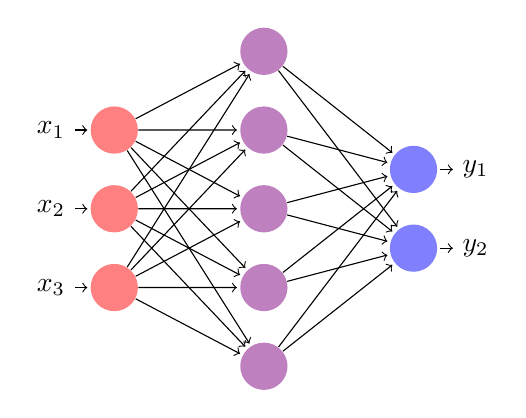
\begin{tikzpicture}

% Input Layer
\foreach \i in {1,...,\inputnum}
{
  \node[circle, 
    minimum size = 6mm,
    fill=red!50] (Input-\i) at (0,-\i) {};
}

% Hidden Layer
\foreach \i in {1,...,\hiddennum}
{
  \node[circle, 
    minimum size = 6mm,
    fill=violet!50,
    yshift=(\hiddennum-\inputnum)*5 mm
  ] (Hidden-\i) at (1.9,-\i) {};
}

% Output Layer
\foreach \i in {1,...,\outputnum}
{
  \node[circle, 
    minimum size = 6mm,
    fill=blue!50,
    yshift=(\outputnum-\inputnum)*5 mm
  ] (Output-\i) at (3.8,-\i) {};
}

% Connect neurons In-Hidden
\foreach \i in {1,...,\inputnum}
{
  \foreach \j in {1,...,\hiddennum}
  {
    \draw[->, shorten >=1pt] (Input-\i) -- (Hidden-\j);	
  }
}

% Connect neurons Hidden-Out
\foreach \i in {1,...,\hiddennum}
{
  \foreach \j in {1,...,\outputnum}
  {
    \draw[->, shorten >=1pt] (Hidden-\i) -- (Output-\j);
  }
}

% Inputs
\foreach \i in {1,...,\inputnum}
{            
  \draw[<-, shorten <=1pt] (Input-\i) -- ++(-0.5,0)
    node[left]{$x_{\i}$};
}

% Outputs
\foreach \i in {1,...,\outputnum}
{            
  \draw[->, shorten <=1pt] (Output-\i) -- ++(0.5,0)
    node[right]{$y_{\i}$};
}

\end{tikzpicture}

  \caption{Et simpelt neuralt netværk}
\end{wrapfigure}
blah blah blah blah blah blah blah blah blah blah blah blah blah blah blah blah blah blah blah blah blah blah blah blah blah blah blah blah blah blah blah blah blah blah blah blah blah blah blah blah blah blah blah blah blah blah blah blah blah blah blah blah blah blah blah blah blah blah blah blah blah blah blah 

\end{document}

\newpage
\printbibliography


\end{document}
